\chapter{Development of a Web Application Programming Interface for Genome Properties Data} \label{micromeda-server}

As discussed in Chapter XXX, one of the core goals of Micromeda is to provide users with an interface for visualizing the presence and absence of genome properties across multiple organisms. The author chose to deliver this software in the form of a web application which takes Micromeda files and uses the data within to generate interactive heat map-based visualizations. The use of a web application has several advantages, and these are discussed in Chapter XXX. Due to the inherent complexity of the information stored within Micromeda files, it was determined that both an in-browser application and supporting server program, called Micromeda-Server, would have to be developed. Such a server would also support the development of some features requested by potential users, such as the ability to download proteins sequences which support the existence of property steps. This chapter will discuss the sever component in detail, including the services it provides and its implementation. The author will further delve into the web application that uses these services in the following Chapter \ref{micromeda-client}.

\section{Overview of Web Servers}

The World Wide Web and associated web applications offer ideal delivery mechanisms for data analysis software such as Micromeda \cite{berners1994world}. In such implementations, users connect to a remote server computer system \footnote{For this document, the term \textbf{server computer system} is used to refer to the physical hardware on which software is running. The term \textbf{server} is used to refer to a software process that provides users or applications with data. A server process may provide data directly to other processes running on the same server computer system or provide data over a network in response to a remote procedure call (RPC) \cite{nelson1981remote}.}. The application is then run within an associated web browser. Most modern websites are, for all intents and purposes, web applications because most use the Javascript programming language \cite{flanagan2006javascript} to script the interactive parts of the site's user interface. Such applications follow a client-server architecture \cite{svobodova1985client} (see \href{en.wikipedia.org/wiki/Client–server\_model}{en.wikipedia.org/wiki/Client–server\_model}) where the code running in the user's browser is called the client. If the client requires external data, it can request this information from a server process running on a server computer system. Clients can request different types of information from a server, including images, videos, files, and stored data. Often the stored data are returned to the client in JSON format \cite{bray2014rfc}. Requests to the server are made, via Hypertext Transfer Protocol (HTTP) \cite{fielding1999hypertext}, using a series of Uniform Resource Locator (URL) addresses \cite{berners1994rfc} (i.e., web addresses) that return specific types of data. These addresses are known as \textbf{endpoints} (Section \ref{endpoints}) and form a web Application Programming Interface (API) (see \href{en.wikipedia.org/wiki/Application\_programming\_interface}{en.wikipedia.org/wiki/Application\_programming\_interface}).

\section{Micromeda-Server Workflow and Implementation} \label{server-workflow}

\begin{figure}[!ht]
  \centering
	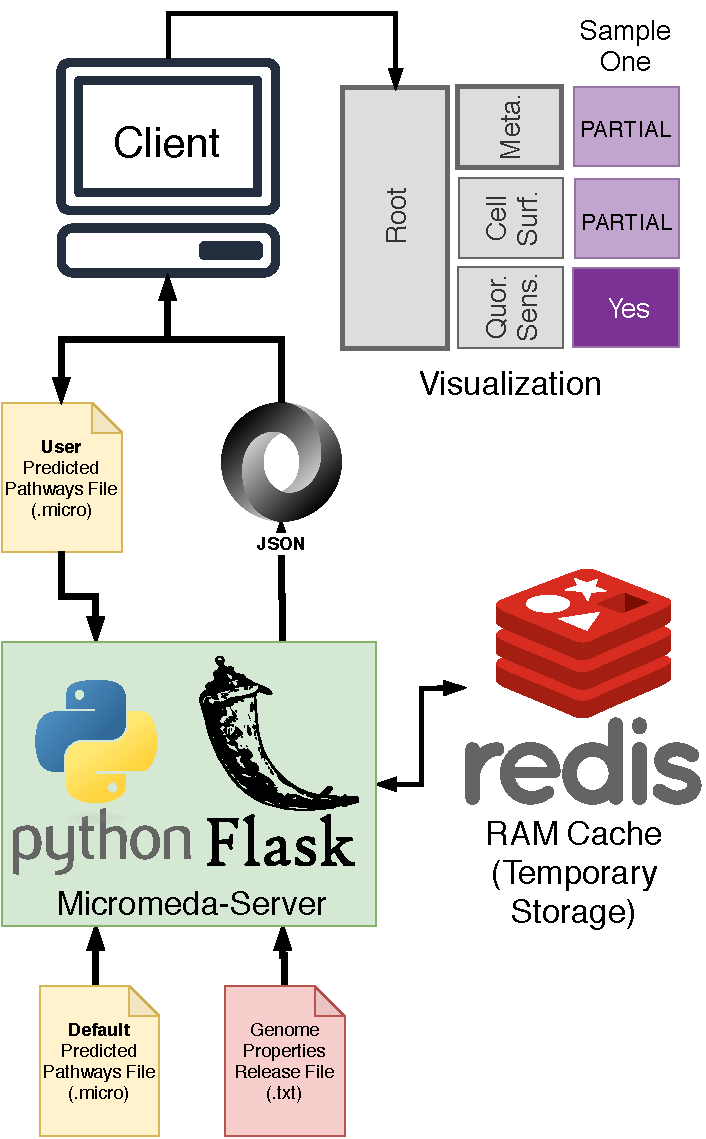
\includegraphics[width=0.60\textwidth]{media/Micromeda-Server.pdf}
	 \caption{Micromeda-Server consists of a server application written in Python using the Flask web framework \cite{grinberg2018flask}. It is supported by a Redis caching server and a series of text files. A genomeproperties.txt file supplies information about the Directed Acyclic Graph (DAG) for the Genome Properties. Micromeda files, either default or uploaded, provide information about property assignments, step assignments, and supporting information across multiple organisms.}
	 \label{fig:micromeda-server}
\end{figure}

\begin{figure}[!ht]
  \centering
	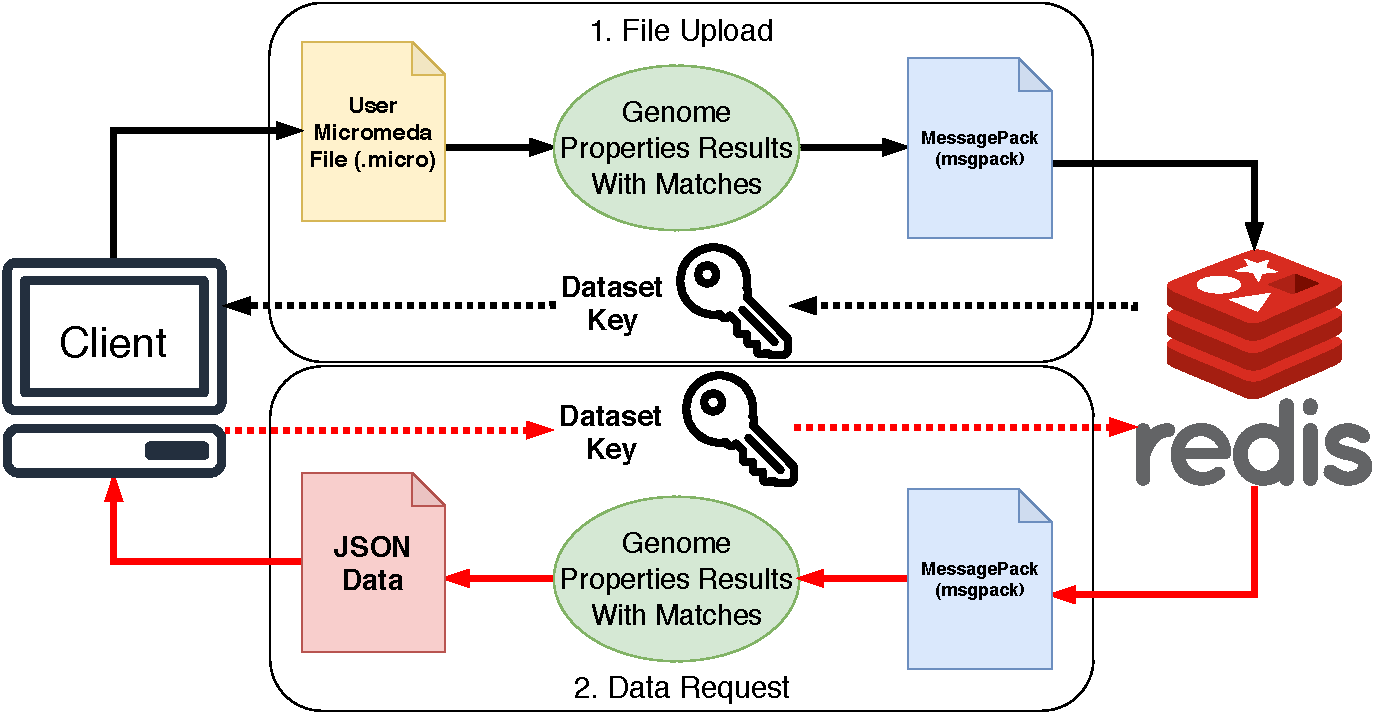
\includegraphics[width=0.80\textwidth]{media/Micromeda-Server-Workflow.pdf}
	 \caption{Micromeda-Server uses uploaded or default Micromeda files to generate GenomePropertiesResultsWithMatches objects. These instantiations are cached in Redis and are reconstituted between API calls. Some endpoints of Micromeda-Server use methods possessed by GenomePropertiesResultsWithMatches objects to produce responses that are sent back to web client applications.}
	 \label{fig:micromeda-server-workflow}
\end{figure}

\begin{figure}[!ht]
  \centering
	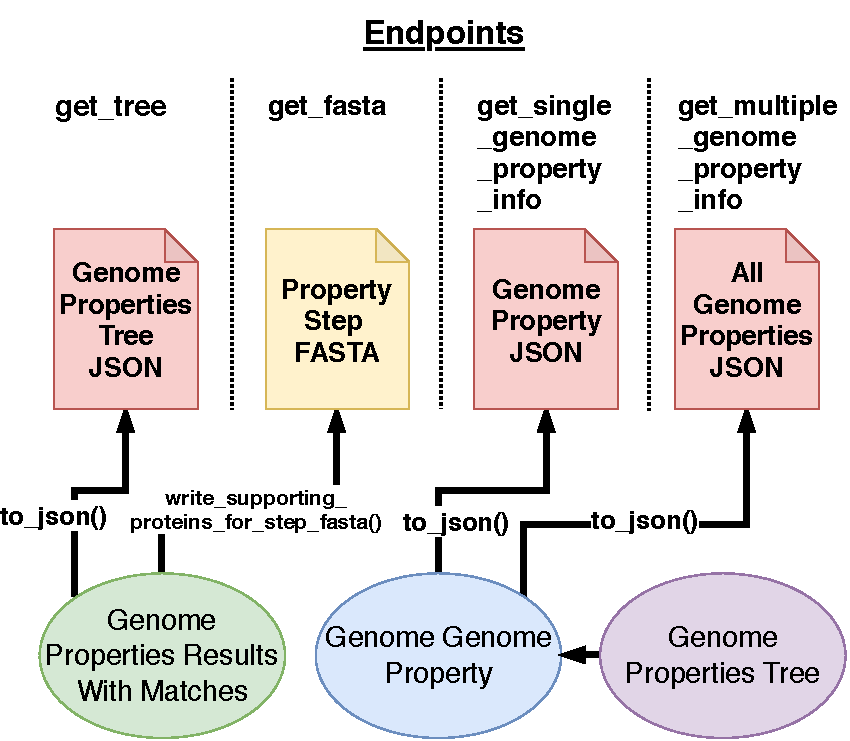
\includegraphics[width=0.70\textwidth]{media/Micromeda-Endpoints.pdf}
	 \caption{JSON documents and FASTA files for individual API endpoints are generated using methods of GenomePropertiesResultsWithMatches objects and the child GenomeProperty objects of GenomePropertiesTree objects.}
	 \label{fig:micromeda-endpoints}
\end{figure}

Micromeda-Server is designed to provide a web API to client applications that require access to information about the Genome Properties database. It also provides an API for accessing temporarily stored property assignments, step assignments, and supporting information for user-supplied datasets. The Micromeda-Server is written in Python and utilizes the Flask web development framework \cite{grinberg2018flask} (Fig. \ref{fig:micromeda-server}) to map Python functions for handling specific web API requests to server URL addresses (i.e., "endpoints"). Information about the Genome Properties database is supplied to Micromeda-Server via a \textbf{genomeProperties.txt} release file (Fig. \ref{fig:micromeda-server} and Section \ref{genome-properties-files}). Property assignments, step assignments, and supporting information for user datasets are supplied via user-uploaded Micromeda files (Fig. \ref{fig:micromeda-server}). These Micromeda files are parsed into GenomePropertyResultsWithMatches objects (Subsection \ref{PropertyResultsWithMatches}) which are later stored in an in-memory Redis cache \footnote{Redis is a server process which provides an in-memory key-value store with a hard-disk drive (HDD) backup \cite{han2011survey}. It allows for the caching of datasets in random-access memory (RAM). Each stored value can subsequently be retrieved from Redis using a key provided during the caching process. These cached objects can even be accessed over the network by processes running on adjacent server computer systems. Redis can also be set up in a distributed cluster configuration across several server computer systems for redundancy and availability. Redis was chosen over some competing caching servers such as Memcached \cite{fitzpatrick2004distributed} due to its capacity for relatively large MessagePack binaries \cite{furuhashi2013messagepack} and its ability to backup data to disk. Disk backup is important because it allows for the safe storage of datasets over time and across high traffic volumes where the server may have run out of RAM if Memcached was used.} in MessagePack format \cite{furuhashi2013messagepack} (Fig. \ref{fig:micromeda-server}, Fig. \ref{fig:micromeda-server-workflow} and Section \ref{msgpack}). In the context of Micromeda-Server, the contents of each uploaded and cached Micromeda file is called a dataset. A single Micromeda file can also be provided to Micromeda-Server during start-up for use as default dataset (Fig. \ref{fig:micromeda-server}). This default dataset is also parsed to a GenomePropertiesResultsWithMatches object and is used to supply data to the API if users upload no Micromeda files. The standard workflow for starting and then using Micromeda-Server is the following:

\begin{enumerate}
  \item Start Micromeda-Server while providing a \textbf{genomeProperties.txt} file and an optional default Micromeda file (Fig. \ref{fig:micromeda-server})
  \item The \textbf{genomeProperties.txt} file is parsed to a GenomePropertiesTree object
  \item The default dataset Micromeda file is parsed to a GenomePropertiesResultsWithMatches object  
  \item The client application sends a user-supplied Micromeda file to the server via the upload endpoint (Fig. \ref{fig:micromeda-server-workflow})
  \item The user-supplied Micromeda files are parsed to a GenomePropertiesResultsWithMatches object which is later stored in the Redis cache in MessagePack format (Fig. \ref{fig:micromeda-server-workflow})
  \item The server supplies the client with a dataset key which is unique to each uploaded Micromeda file (Fig. \ref{fig:micromeda-server-workflow})
  \item The client can later supply this dataset key to the server during proceeding API requests to get information from the previously uploaded Micromeda file (Fig. \ref{fig:micromeda-server-workflow})
  \item If the client provides no dataset key then the server supplies information about the default dataset during API requests
\end{enumerate}

Each GenomePropertiesResultsWithMatches object cached to Redis is given a Time To Live (TTL) value \cite{gwertzman1996world} (see \href{en.wikipedia.org/wiki/Time\_to\_live}{en.wikipedia.org/wiki/Time\_to\_live}). Users can set this value for any period, such as minutes or days. After the TTL of the cached object is exceeded, it is flushed from the cache; the user will then have to re-upload their Micromeda file. The default TTL used is two hours. During each API request, if a dataset key is provided, the MessagePack-formatted GenomePropertiesResultsWithMatches object is grabbed from the cache and reconstituted into its original form (Fig. \ref{fig:micromeda-server-workflow}). During the API call this reconstituted GenomePropertiesResultsWithMatches object's methods are used to supply data to the client  (Fig. \ref{fig:micromeda-server-workflow} and Fig. \ref{fig:micromeda-endpoints}). Further details on these endpoints are provided in Section \ref{endpoints}.

Micromeda files contain information about both assignments and supporting information used in their creation. This supporting information, such as proteins sequences, can take up substantial disk space. Permanently storing such information would be prohibitive in terms of both hardware and maintenance costs. In response, Micromeda-Server was designed to store uploaded datasets temporarily. If users deploying Micromeda-Server want to store data more permanently, they can change the TTL value mentioned above to a value that emulates permanent storage, such as years. Micromeda-Server does not have a user login system \footnote{A user login system is very complex to build and maintain. Code for tracking usernames, passwords, and emails must be generated. Code for handling logins, logout, and passwords changes in a secure manner would also have to be implemented.} and uploads to the server are done anonymously. There is no way to track which uploaded datasets belong to what users. This lack of tracking is another reason for not permanently storing datasets because there would be no way to delete permanently stored datasets for one user but not others.

\section{Use of Redis for Dataset Caching} \label{redis-caching}

Python, due to limitations in its default cPython interpreter \cite{van1995python}, is only capable executing one compute thread \cite{saltzer1966traffic} (see \href{en.wikipedia.org/wiki/Thread\_(computing)}{en.wikipedia.org/wiki/ \\ Thread\_(computing)}) at a time \cite{beazley2010understanding}. This limitation causes problems for web server APIs that are required to handle multiple requests from clients simultaneously. In response, the majority of Python web frameworks, which provide boilerplate code for writing API endpoints, are designed to run multiple copies of the Python code, which handles endpoint requests (Fig. \ref{fig:client-processing}). Flask is one such framework \cite{grinberg2018flask}. These codes are run in separate processes (see \href{en.wikipedia.org/wiki/Thread\_(computing)\#Threads\_vs.\_processes}{en.wikipedia.org/wiki/Thread\_(computing)\#Threads\_vs.\_processes}) and do not share a memory space (Fig. \ref{fig:client-processing}). Thus, any in-memory objects created for one API request are not shared with the others (Fig. \ref{fig:client-processing}). Also, there is no guarantee that subsequent API requests from a single web client will be mapped repeatedly to the same API server process (Fig. \ref{fig:client-processing}). This lack of mapping causes a problem as a GenomePropertiesResultsWithMatches object created by an upload would be stored in only one process and would not be available to other processes that future client requests may call (Fig. \ref{fig:client-processing}). One way of circumventing this process isolation issue is to store data to be shared between web server processes in an external process that is used as a cache (Fig. \ref{fig:micromeda-server-workflow} and Fig. \ref{fig:client-processing}). This way, all web API processes have one place where they access shared data. Micromeda-Server uses Redis as this caching process. Redis is a caching server that stores keyed data RAM. 

Micromeda-Server uses Redis to cache GenomePropertiesResultsWithMatches objects, in MessagePack format, for use by multiple request handling processes (Fig. \ref{fig:micromeda-server-workflow} and Fig. \ref{fig:client-processing}). Micromeda-Server generates these GenomePropertiesResultsWithMatches objects from Micromeda files uploaded to the server. During API requests where the client wants data from a specific dataset, API processes can pull MessagePack formatted GenomePropertiesResultsWithMatches objects from the Redis cache, reconstitute them and then use their methods to gather data for a response (Fig. \ref{fig:micromeda-server-workflow} and Fig. \ref{endpoints}). Rapid serialization of MessagePack to GenomePropertiesResultsWithMatches objects allows for this design pattern (see Subsection \ref{messagepack-performance}).

\begin{figure}[!ht]
  \centering
	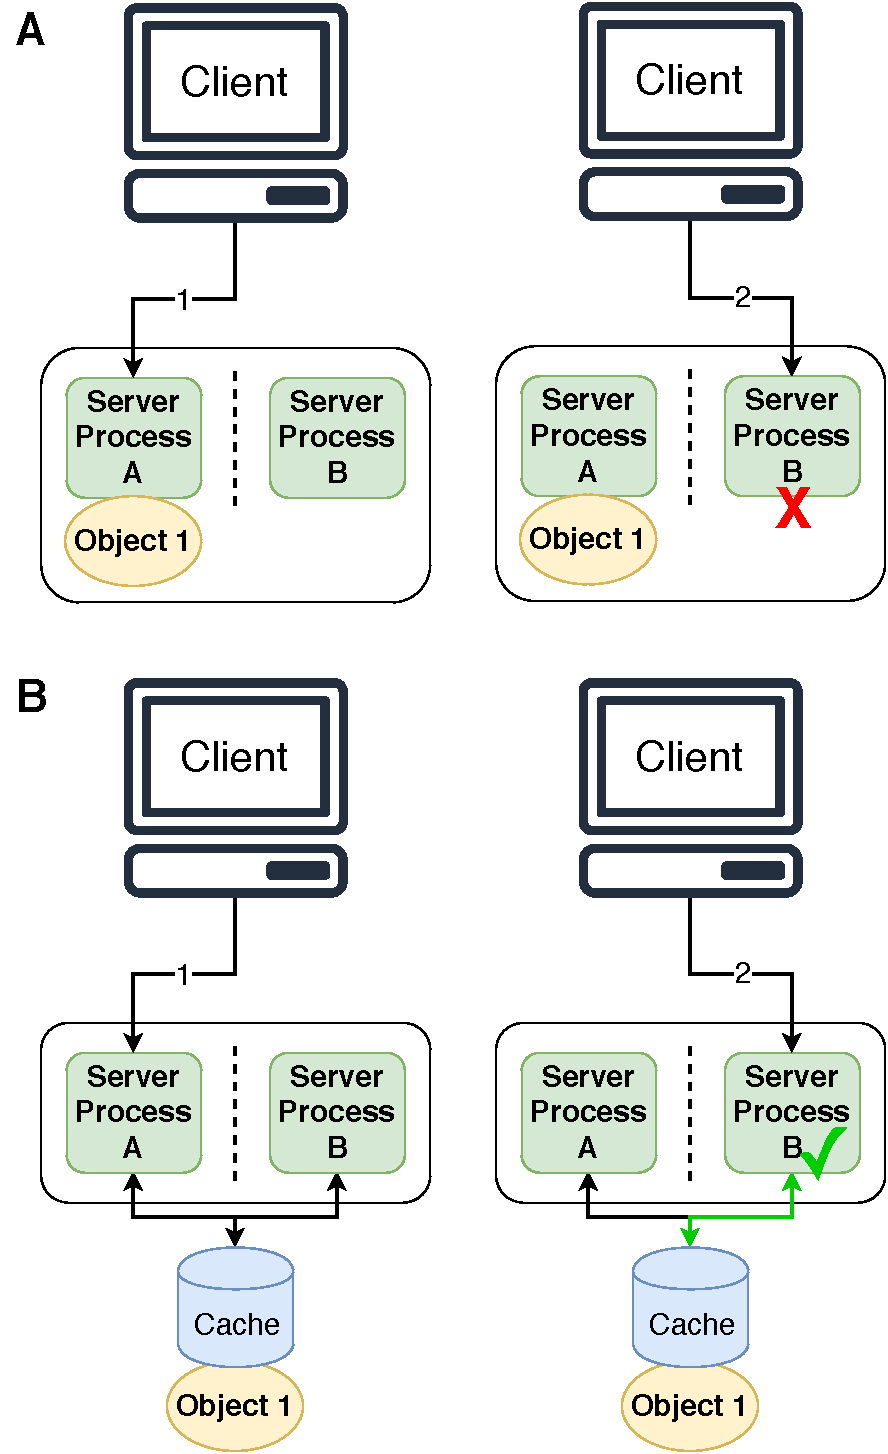
\includegraphics[width=0.50\textwidth]{media/Client-Processing.pdf}
	 \caption{Requests directed towards Python web APIs are spread out among a series of process. (A) These processes cannot share data directly. (B) Data to be shared between processes must be stored in a third process, such as a cache or database.}
	 \label{fig:client-processing}
\end{figure}

\section{Application Programming Interface Endpoints} \label{endpoints}

Micromeda-Server provides several endpoints for supplying web clients with information about individual genome properties and information from uploaded Micromeda files. These endpoints were written using the Flask Python web framework \cite{grinberg2018flask} and are represented by \textbf{clean URLs} (see \href{en.wikipedia.org/wiki/Clean\_URL}{en.wikipedia.org/wiki/Clean\_URL}) where some information that would normally be stored as HTTP GET parameters are stored in the URL path (Fig. \ref{fig:endpoint-url}). Flask was chosen due to its simplicity as compared to more comprehensive frameworks such as Django \cite{holovaty2009definitive}. The endpoints also follow a representational state transfer (REST) architecture \cite{fielding2000representational} (see \href{en.wikipedia.org/wiki/Representational\_state\_transfer}{en.wikipedia.org/wiki/Representationa \_state\_transfer}). These endpoints and their implementation are summarized in Table \ref{tab:endpoints}, Fig. \ref{endpoints}, Fig. \ref{fig:endpoint-url}, and detailed in subsections below.

\begin{figure}[!ht]
  \centering
	
\includegraphics[width=\textwidth]{media/Coloured-Endpoint.pdf}
	 \caption{The URL above is used to download a FASTA file for containing the top proteins (i.e., those with lowest E-value domains) that support GenProp0526 step one for dataset FXDABADS. The URL path variables are in blue and the HTTP GET parameters are in green.}
	 \label{fig:endpoint-url}
\end{figure}

\begin{longtable}{|p{1.6cm}|p{2.5cm}|p{1.4cm}|p{2.2cm}|p{2.2cm}|p{4cm}|}
\caption{Micromeda's server component provides web applications with five endpoints where they can request data about individual genome properties, upload Micromeda files, and request information about stored assignment databases.}
\label{tab:endpoints}\\
\hline
\textbf{Python Function Name} & \textbf{Endpoint URL} & \textbf{HTTP Request Types} & \textbf{URL Path Variables} & \textbf{GET Parameter Variables} & \textbf{Return Value} \\ \hline
\endfirsthead
%
\multicolumn{6}{c}%
{{\bfseries Table \thetable\ continued from previous page}} \\
\hline
\textbf{Python Function Name} & \textbf{Endpoint URL} & \textbf{HTTP Request Types} & \textbf{URL Path Variables} & \textbf{GET Parameter Variables} & \textbf{Return Value} \\ \hline
\endhead
%
upload & /upload & GET, POST & None & None & JSON containing a dataset key that can be used by future API requests to access information from the uploaded Micromeda file \\ \hline
get\_tree & /genome \_properties \_tree & GET & None & dataset\_key (optional) & A JSON tree representing all properties in the current Genome Properties database with each node annotated with a list of YES, NO, PARTIAL assignments for each organism in a dataset. \\ \hline
get\_single \_genome \_property \_info & /genome \_properties/ \textless{}string: property\_id\textgreater{} & GET & property\_id & None & JSON containing information about a genome property such as a description of it and a list of equivalent records from other databases (e.g. KEGG \cite{kawashima2003kegg}, MetaCyc \cite{karp2002metacyc}) \\ \hline
get \_multiple \_genome \_property \_info & /genome \_properties & GET & None & None & A JSON array containing information about all genome properties in the database. Each property is given a description and a list of equivalent records from other databases (e.g. KEGG, MetaCyc) \\ \hline
get\_fasta & /fasta/ \textless{}string: property\_id\textgreater{}/ \textless{}int:step \_number\textgreater{} & GET & property\_id, step\_number & dataset\_key (optional), all (optional) & A FASTA file containing either all or the top proteins (i.e., those with the lowest E-value domain annotations) supporting the existence of a given property step. A dataset key can be provided to specify a dataset. \\ \hline
\end{longtable}

\subsection{The Upload Endpoint} \label{endpoint-upload}

This API endpoint accepts the client upload of a Micromeda file and returns a hexadecimal encoded universally unique identifier (UUID) key \cite{leach2005universally} (see \href{en.wikipedia.org/wiki/Universally\_unique\_identifier}{en.wikipedia.org/wiki/ Universally\_unique\_identifier}) to the client. After upload, the Micromeda file is parsed and transformed into a GenomePropertiesResultsWithMatches object. This object is then serialized to MessagePack using the object's \textbf{to\_msgpack} function (Table \ref{tab:genomepropertyresultswithmatches})) and the resulting binary is cached in Redis using the Redis Python library \cite{mccurdy_2019} (Fig. \ref{fig:micromeda-server-workflow}). During the previous process, a UUID, to be used as a dataset key, is generated using Python's built in UUID generation function \cite{PythonUUID}. This UUID is used as the key for accessing the MessagePack serialization stored in the Redis cache (Fig. \ref{fig:micromeda-server-workflow}). Micromeda-Server returns the key to the client application in response to the file upload. The client can provide this key to other API endpoints to receive data from the uploaded Micromeda file (Fig. \ref{fig:micromeda-server-workflow}). 

\subsection{The Get\_Tree Endpoint} \label{get-tree}

The \textbf{get\_tree} endpoint provides the client with a JSON tree representing all properties and steps in Genome Properties database (Fig. \ref{fig:tree-json}). This tree represents parent-child relationships between properties. Step nodes are also attached to their parent genome property nodes and act as leaves (Fig. \ref{fig:tree-json}). Note that this endpoint returns a tree rather than a DAG (Fig. \ref{fig:tree-json}). In this tree, properties which would have had two parents in the Genome Properties DAG (Section XXX) are duplicated (Fig. fig:tree-json). Each property and step node in the tree is annotated by a list of assignments of support (i.e., YES, NO, PARTIAL), one for each sample in a previously uploaded or default Micromeda file (Fig. \ref{fig:tree-json}). The \textbf{Get\_Tree} endpoint can take a \textbf{dataset\_key} HTTP GET parameter variable (Table \ref{tab:endpoints}). If a dataset key generated by the previous upload of a Micromeda file is assigned to this variable, then the assignments of support stored in the key's associated Micromeda file are returned. The dataset key is used to reconstitute a GenomePropertiesResultsWithMatches object, representing the uploaded Micromeda file, from the Redis cache. The GenomePropertiesResultsWithMatches object's \textbf{to\_json} method (Table \ref{tab:genomepropertyresultswithmatches}) is called to generate the above tree JSON. This JSON returned to the client by the endpoint. If no dataset\_key is provided to the endpoint, GenomePropertiesResultsWithMatches object of the default Micromeda is used to generate the tree JSON using the same method.

\begin{figure}[!ht]
  \centering
	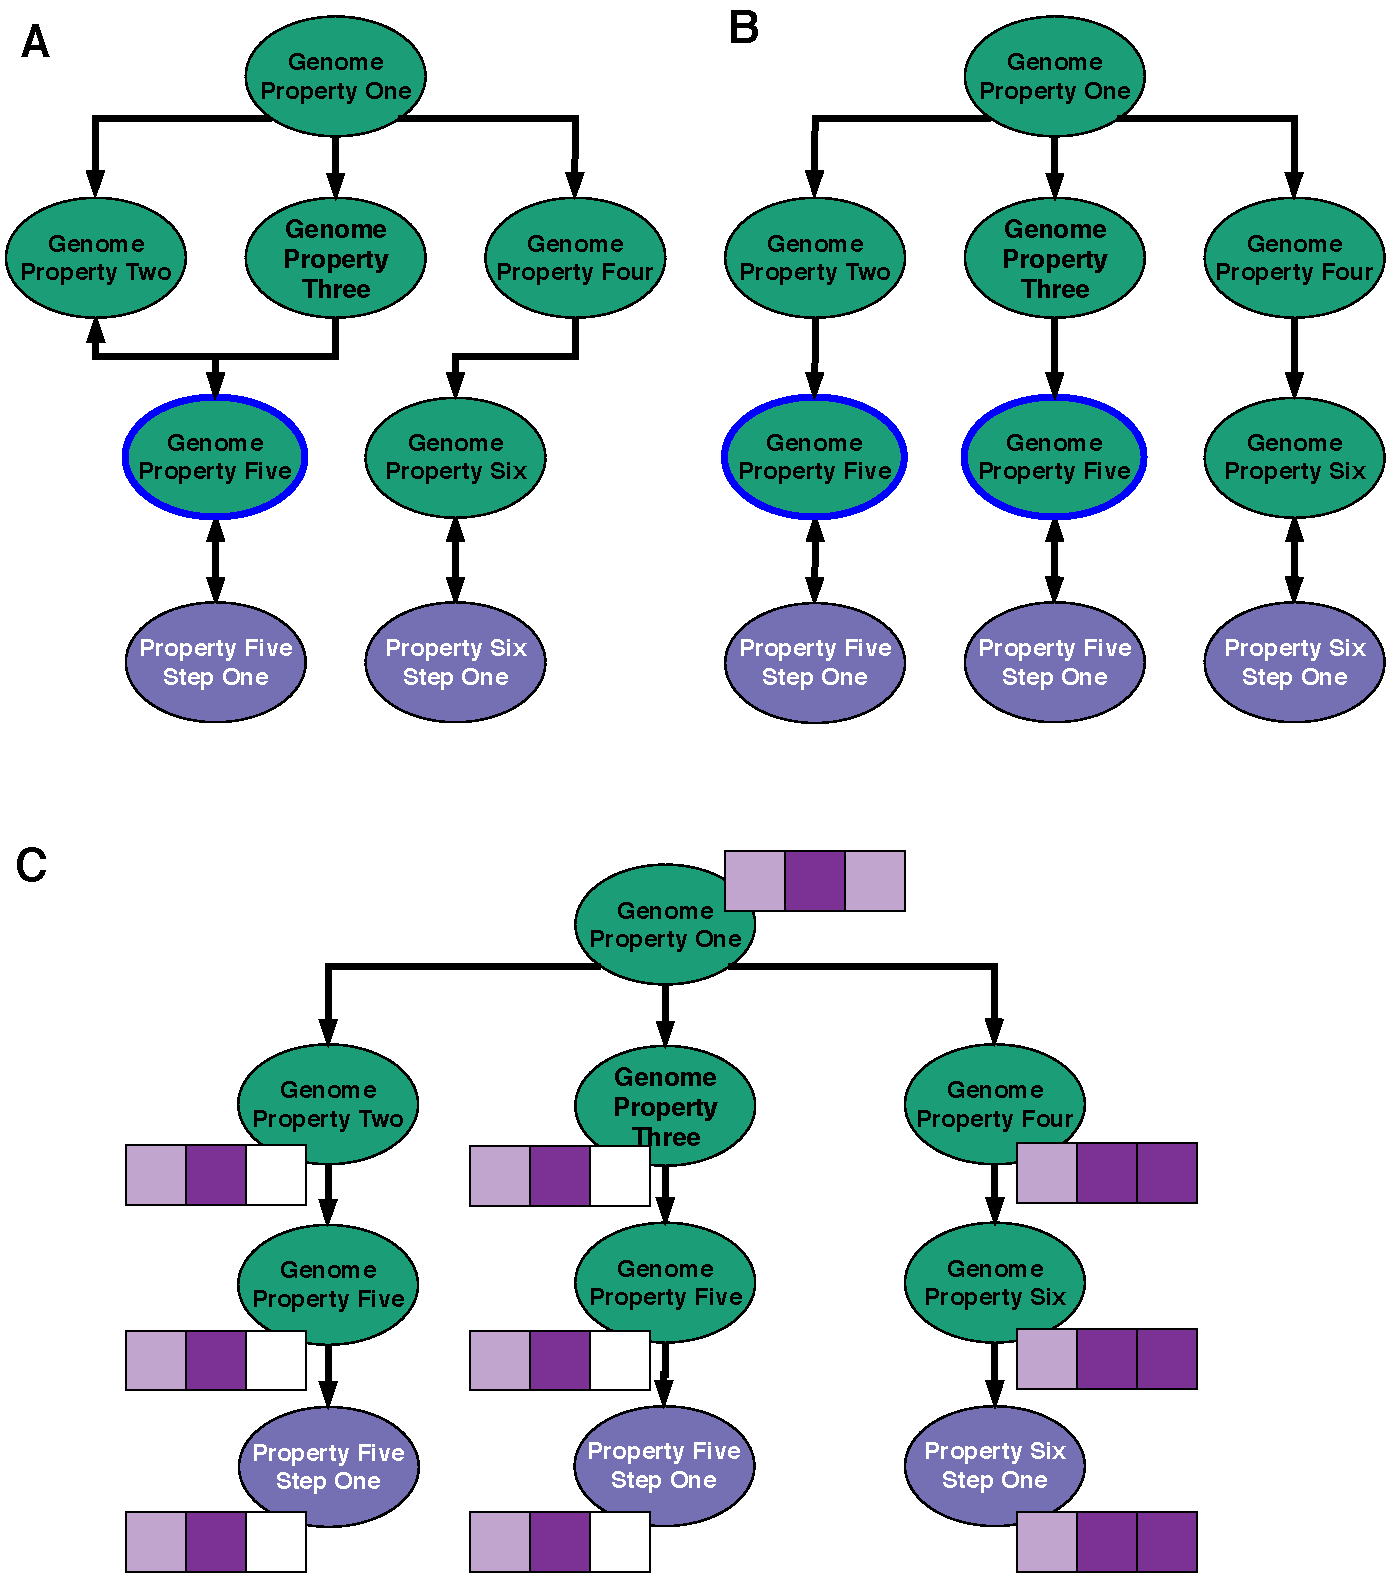
\includegraphics[width=0.70\textwidth]{media/Tree-JSON.pdf}
	 \caption{(A and B) The JSON document created by the Get\_Tree endpoint forms a tree (right), not a DAG (left). (B) In this tree, nodes can be repeated. (C) In this JSON document, each node is tagged with a list YES (Dark Purple), PARTIAL (Light Purple), and NO (White) assignments.}
	 \label{fig:tree-json}
\end{figure}


\subsection{The Get\_Single\_Genome\_Property\_Info Endpoint} \label{get-property-info-endpoint}

The \textbf{get\_single\_genome\_property\_info} endpoint takes a genome property identifier as a URL parameter (Table \ref{tab:endpoints}). This genome property identifier is used query for a matching GenomeProperty object (Section \ref{genome-property-class}), representing the property whose identifier is specified, from a global GenomePropertiesTree object (Section \ref{GenomePropertiesTree-Class}) created on Micromeda-Server's start up (Section \ref{server-workflow}). If found, this GenomeProperty object's \textbf{to\_json} method (Table \ref{tab:genome-property-object}) is called to create a JSON document containing property information that is returned by the endpoint. This JSON document includes the property name, property description, and a list of equivalent records from other databases (Table \ref{tab:genome-property-object}).

\subsection{The Get\_Multiple\_Genome\_Property\_Info Endpoint}

When the \textbf{get\_multiple\_genome\_property\_info} endpoint is called, the \textbf{to\_json} method (Table \ref{tab:genome-property-object}) is called on every GenomeProperty object (Section \ref{genome-property-class}), which is a child of the GenomePropertiesTree object (Section \ref{GenomePropertiesTree-Class}) created on Micromeda-Server start up. Each of the JSON strings generated are placed into a list in a single larger JSON document, which is then returned by the endpoint. 

\subsection{The Get\_Fasta Endpoint} \label{get-fasta-endpoint}

The \textbf{get\_gasta} endpoint is used to send the client a FASTA file containing protein sequences that support the existence of a property step across multiple organisms in a specific uploaded dataset. The URL path of requests to this endpoint includes the genome property identifier and step number of the property step required to generate a FASTA file. The FASTA file can either contain all proteins that support the existence of a property step or only those with the lowest E-value for the InterPro domain offering support for a given step. These proteins are known as the \textbf{"top"} hits. The contents of the returned file is controlled by the presence of a HTTP GET parameter called \textbf{all} (Fig. \ref{fig:endpoint-url}). If \textbf{all} is set to true, then a FASTA file containing all proteins that support a step is returned. Otherwise, a FASTA file containing only the lowest E-value proteins is returned. Like the Get\_Tree endpoint, this endpoint also accepts a \textbf{dataset\_key} HTTP GET parameter (Fig. \ref{fig:endpoint-url}). The value of this variable is used to reconstitute a GenomePropertiesResultsWithMatches object representing a previously uploaded Micromeda file (Fig. \ref{fig:micromeda-server-workflow}). This object's \textbf{write\_supporting\_proteins\_for\_step\_fasta} function (Table \ref{tab:genomepropertyresultswithmatches}) is used generate the FASTA file, which is sent to the client.

\section{Micromeda Server Performance} \label{micromeda-server-performance}

The performance of Micromeda's endpoints was tested using a Micromeda file generated from the protein sequences and InterProScan annotations of \textit{Chlorobium chlorochromatii} CaD3 (NCBI Taxonomy ID 340177) and \textit{Pelodictyon luteolum} DSM 273 (NCBI Taxonomy ID 319225). When this file was sent to the \textbf{upload} endpoint of Micromeda-Server it was parsed and added to the Redis cache in 11.3 \textpm 2 s. The \textbf{get\_tree} endpoint could create a genome property tree from this cached Micromeda file in 9.4 \textpm 4 s. The \textbf{get\_fasta} endpoint could generate a FASTA file with the top supporting proteins for GenProp0633 step number two in 33 \textpm 4 ms. The property information JSON file could be generated for GenProp0633 by the \textbf{get\_single\_genome\_property\_info} endpoint in 7 \textpm 2 ms. The \textbf{get\_multiple\_genome\_property\_info} can generated JSON files for all properties in 23 \textpm 5 ms. The slow execution time of the \textbf{upload} and \textbf{get\_tree} endpoints was a result of latency in client applications. For example, there was a noticeable delay in the rendering of visualizations in Micromeda's client application. Thus the performance of these endpoints should be optimized and potential optimizations are discussed in Section \ref{micromeda-server-improvements}.

\section{Micromeda Server Deployments} \label{micromeda-server-deployments}

It is common to deploy web servers in different configurations depending on the expected request volume. Choosing the optimal configuration becomes important for Micromeda-Server because it is written using the Flask web framework \cite{grinberg2018flask}. Flask is single-threaded and high performance can only be achieved by running multiple copies of Micromeda-Server's Python code in parallel (as discussed in Section \ref{redis-caching}). These copies can be run on a single computer or across a cluster. Redis can also be run in cluster configuration. Three deployment strategies of increasing size will be discussed below. 

\subsection{Development and Single User Deployment}

If a user wishes to install and run Micromeda-Server on their desktop or laptop and only needs to visualize one dataset at a time, then a very simplified deployment strategy can be used (Fig. \ref{fig:micromeda-small-deploy}). This deployment uses Flask's built in development HTTP server to respond to requests. The server is activated when Micromeda-Server's Python script is run directly from a command-line interface (\href{en.wikipedia.org/wiki/Command-line\_interface}{en.wikipedia.org/wiki/Command-line\_interface}). This single-user deployment is slow and can only handle single requests from single clients. In this configuration, Redis is not required, and users must tell Micromeda-Server to use their dataset (i.e., a Micromeda file) as its default (Fig. \ref{fig:micromeda-small-deploy}). The upload endpoint is also turned off. This deployment method is similar to the one used by Anvio's Metagenome Assembled Genome (MAG) visualization and refinement server \cite{eren2015anvi}. The single-user deployment configuration is also useful for developers who want to test newly developed features or bug fixes.

\begin{figure}[!ht]
  \centering
	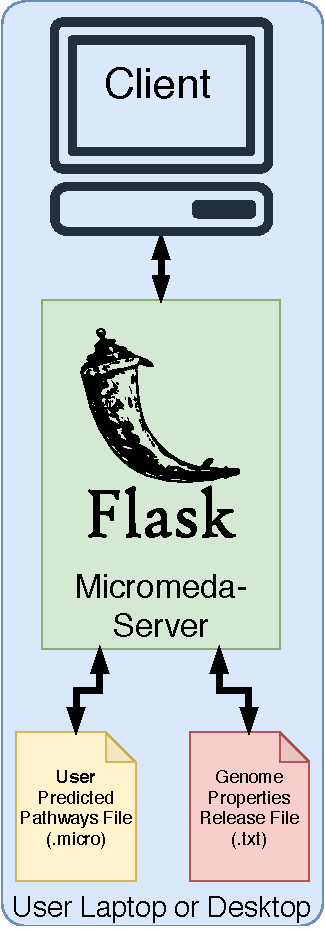
\includegraphics[width=0.30\textwidth]{media/micromeda-simple-deployment.pdf}
	 \caption{For the development use or deployment to laptop and desktops, Micromed-Server can use Flask's builtin HTTP server, a genomeProperties.txt file, and a Micromeda file supplied on the server on startup to handle requests from a single client.}
	 \label{fig:micromeda-small-deploy}
\end{figure}

\subsection{Single Server Deployment} \label{single-server-micromeda-deployment}

If a user requires Micromeda-Server to handle multiple users simultaneously, such as would be the case if it was installed on a server computer system, a larger deployment must be used (Fig. \ref{fig:micromeda-medium-deploy}). This deployment type adds additional software layers that increase Micromeda-Server's scalability. As discussed in previous sections, multiple copies of Micromeda-Server's Python code must be run simultaneously to handle multiple client requests. This technique is done by putting the Micromeda-Server under the command of a master HTTP server that can route traffic to multiple copies of the code in separate processes (Fig. \ref{fig:micromeda-medium-deploy}). Such master HTTP servers include the Apache \cite{fielding1997apache} and NGINX \cite{reese2008nginx} HTTP servers. This master server handles the parsing of HTTP requests. In addition to the master server, a middleware component must also be used and handles the spawning of multiple copies of Micromeda-Server processes (Fig. \ref{fig:micromeda-medium-deploy}). Examples of software that can be used as middleware are uWSGI \cite{2019uwsgi} and gunicorn \cite{chesneau_2018}. All three components (i.e., HTTP server, middleware server, and Micromeda-Server) communicate via Web Server Gateway Interface (WSGI) protocol \cite{gardner2009web}. As noted in Section \ref{redis-caching}, Redis has to be used to cache GenomePropertiesResultsWithMatches objects between requests in this deployment type. All components of the above server are deployed on the same server computer system (Fig. \ref{fig:micromeda-medium-deploy}).

\begin{figure}[!ht]
  \centering
	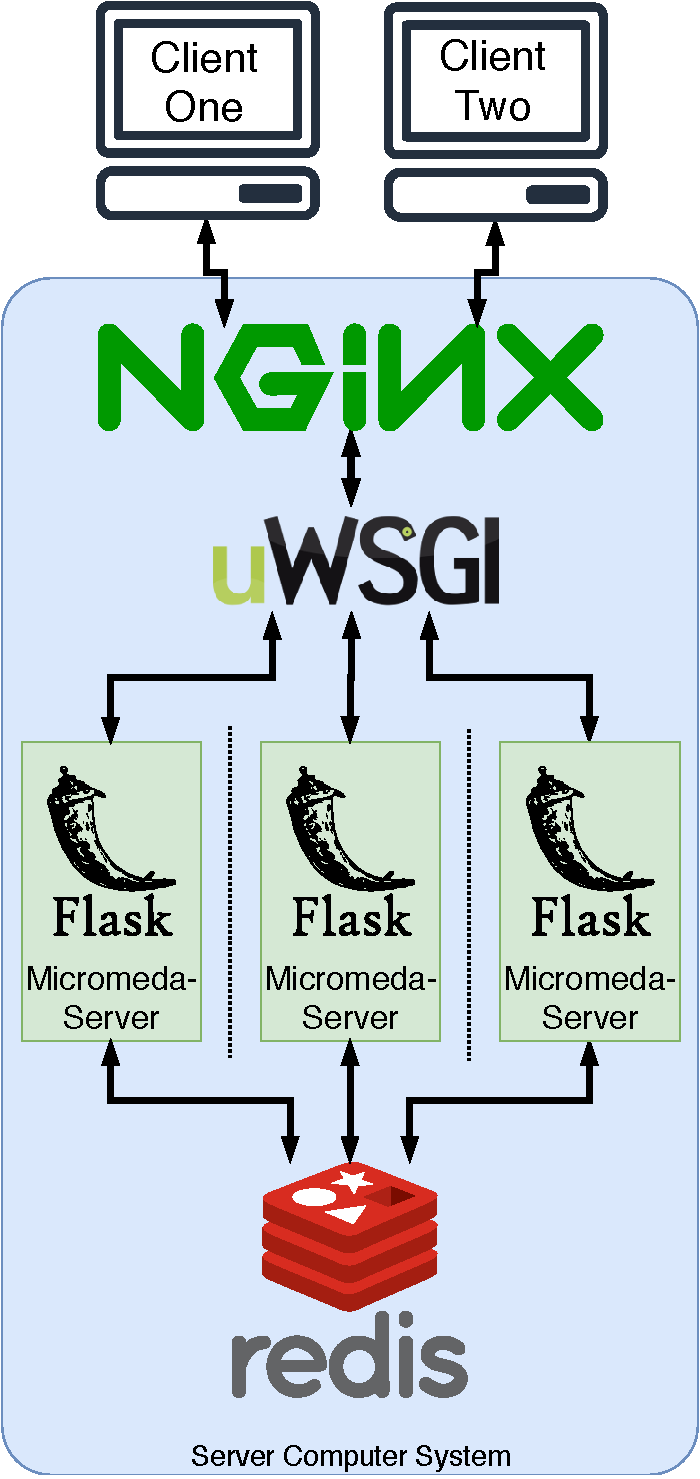
\includegraphics[width=0.40\textwidth]{media/micromeda-medium-deployment.pdf}
	 \caption{When deployed to handle traffic of multiple clients, Micromed-Server's Python code is placed behind an HTTP server and uWSGI middleware server. Multiple copies of the Python code can then be run simultaneously. Redis is used to provide shared data between these processes. The genomeProperties.txt files and default Micromeda files are still used but were omitted from the diagram for simplicity.}
	 \label{fig:micromeda-medium-deploy}
\end{figure}

\subsection{Multiple Server Deployment} \label{multi-server-micromeda-deployment}

For a large number of simultaneous users, Micromeda-Server may need to be scaled horizontally to multiple servers (Fig. \ref{fig:micromeda-large-deploy}). This scaling is done by placing a load balancer \footnote{A load balancer (see \href{en.wikipedia.org/wiki/Load\_balancing\_(computing)}{en.wikipedia.org/wiki/Load\_balancing\_(computing)} is a piece of software that routes HTTP traffic between a cluster of web servers. NGINX \cite{reese2008nginx} can be configured as a load balancer (Fig. \ref{fig:micromeda-medium-deploy}).} out front of multiple copies of the previous deployment running on separate server computer systems (Fig. \ref{fig:micromeda-large-deploy}). Redis can also be run on a single server computer system or computing cluster (Fig. \ref{fig:micromeda-large-deploy}). Such multiple server deployment strategies can be scaled horizontally by adding new server computer systems to the deployment (Fig. \ref{fig:micromeda-large-deploy}). These new server computer systems can handle increases in request volume.

\begin{figure}[!ht]
  \centering
	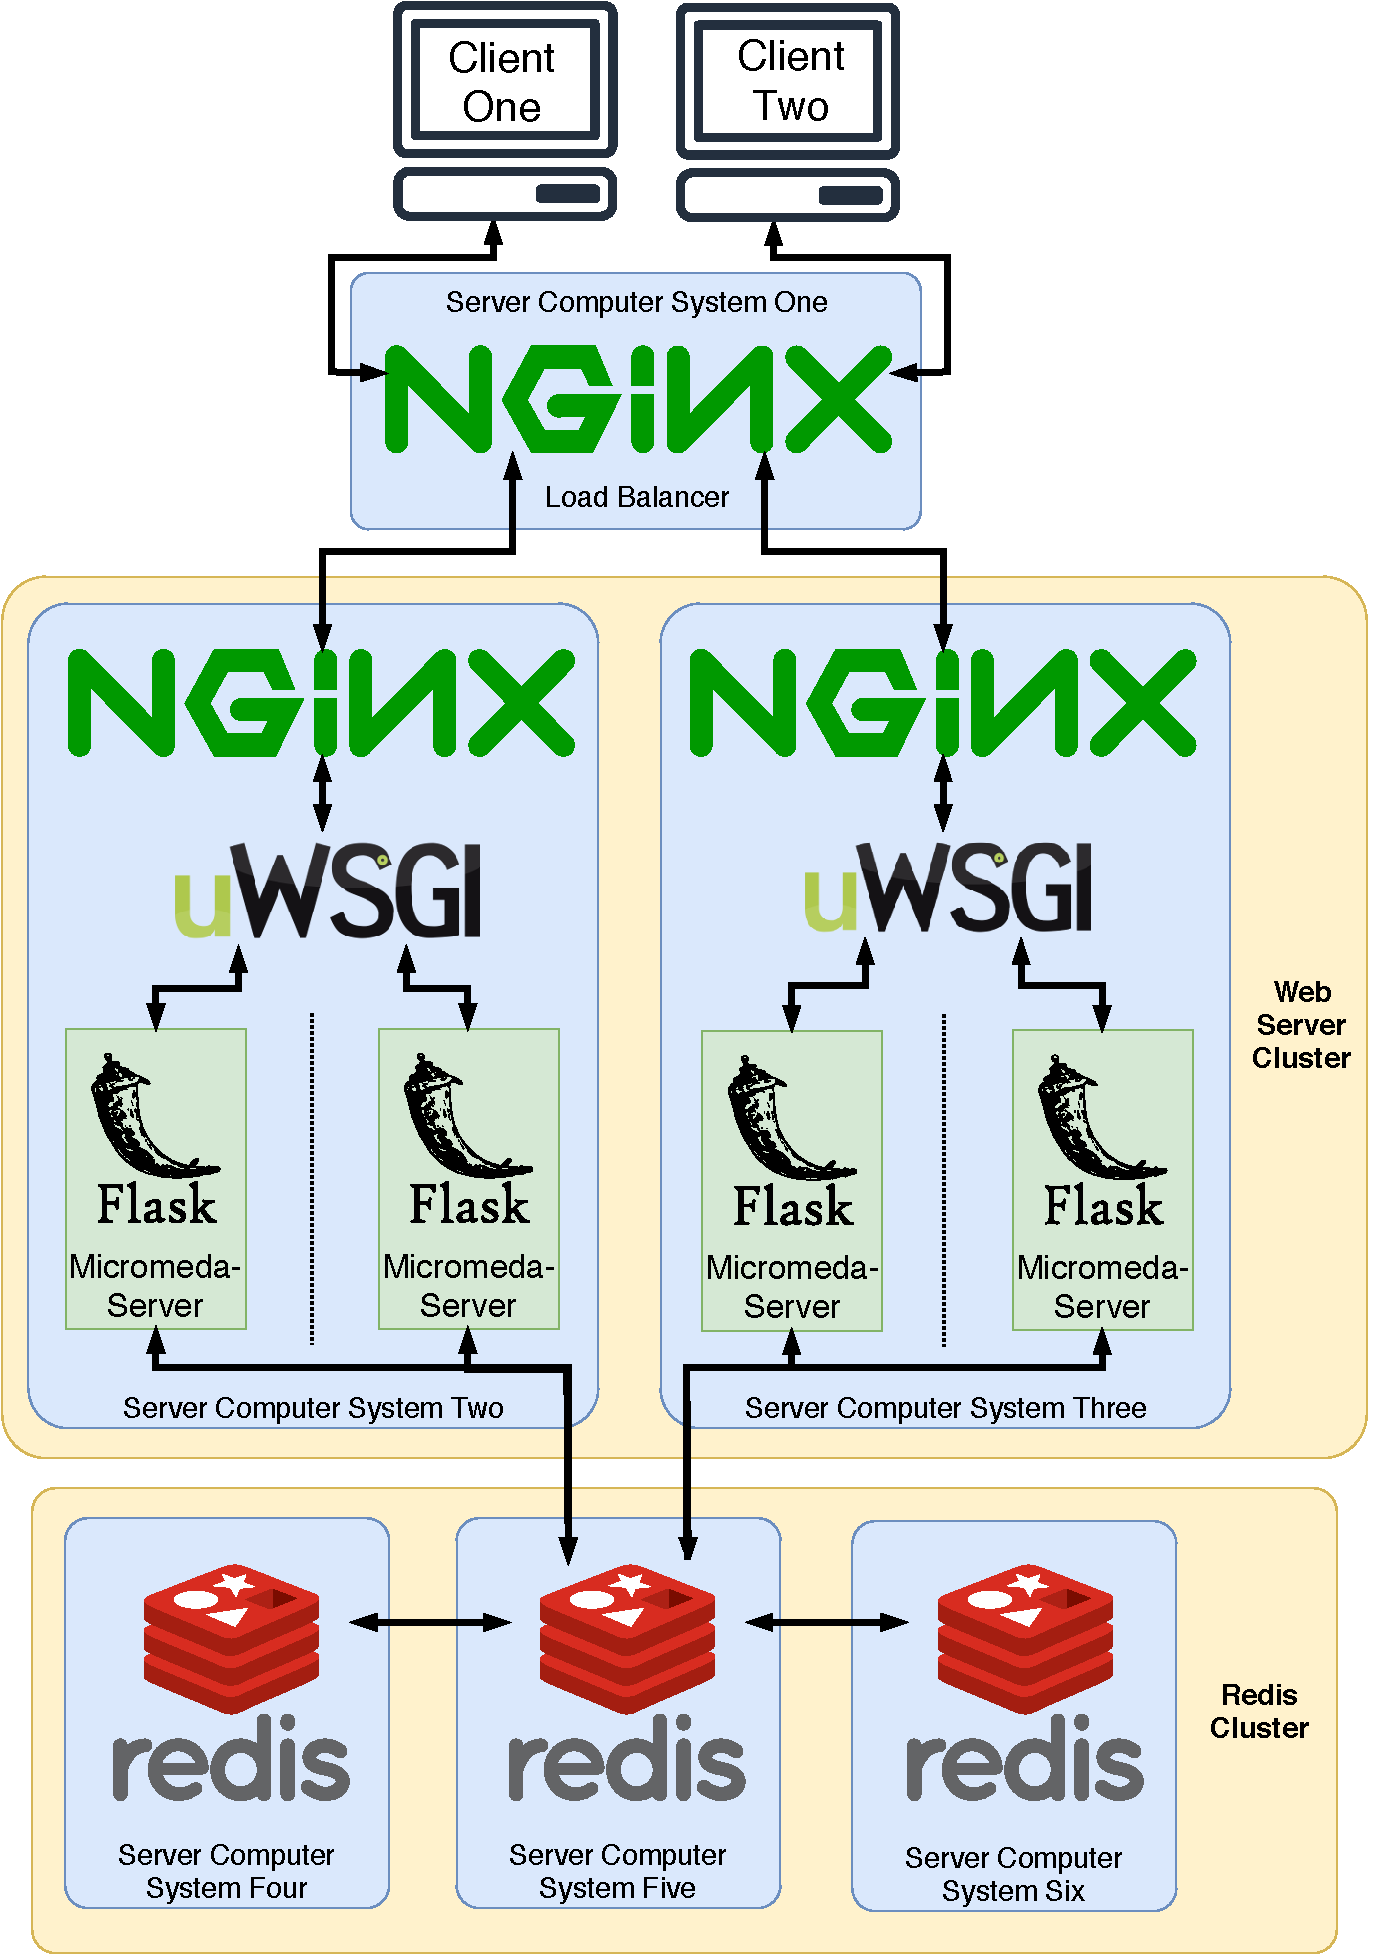
\includegraphics[width=0.50\textwidth]{media/micromeda-heavy-deployment.pdf}
	 \caption{When Micromeda is required to scale to handle hundreds or thousands of simultaneous users, its workload must be spread out across multiple caching and web server computer systems. The performance of such deployments can be increased by adding hardware to either of the caching or web server clusters. A copy of the genomeProperties.txt file and default Micromeda file would be stored on each computer in the web server cluster and they have been omitted from the diagram for simplicity.}
	 \label{fig:micromeda-large-deploy}
\end{figure}

\subsection{Cloud Platform As A Service (PaaS) Deployment}

Various cloud computing corporations have developed Platform as a Service (PaaS) \cite{lawton2008developing} products (see \href{en.wikipedia.org/wiki/Platform\_as\_a\_service}{en.wikipedia.org/wiki/Platform\_as\_a\_service}) that help users scale Python web applications without having to spend the time setting up complex multiple server deployments as discussed above. These PaaS, such as Google App Engine (\href{cloud.google.com/appengine}{cloud.google.com/ appengine}) or Heroku (\href{heroku.com}{heroku.com}), provide the simplicity of a single user deployment with the scalability of multiple server deployments. They do this by only requiring the developers to upload their Flask Python code and then automate the rest of the deployment process. For example, load balancers and multiple copies of request handling processes are spun up by such platforms automatically. Such platforms perform these tasks in the background and invisibly to the developer who uploaded the code. PaaS can also be set up to pull new versions of applications directly from their Github repository upon software release, allowing for the continuous update of the deployment's Python code to the latest version. PaaS systems also allow for the deployment of Redis clusters, for example, Google's Cloud Memorystore (see \href{cloud.google.com/memorystore/}{google.com/memorystore}).

\section{Future Improvements} \label{micromeda-server-improvements}

Micromeda-Server currently provides endpoints for all the information needed by Micromeda's web-based visualization client. However, in addition to the existing endpoints, new endpoints could be made that would provide new data for future versions of this client, allowing it to have expanded functionality. Performance optimizations for the existing endpoints could also be made, which could reduce latency in the client's user interface by reducing the time spent waiting for responses from Micromeda-Server. Improvements to Micromeda-Server's existing endpoints and a potential new endpoint are discussed below.

\subsection{Improving Performance of the Upload Endpoint}

The \textbf{upload} endpoint takes a Micromeda file and saves its contents to a Redis cache. This endpoint was shown to have poor performance (see Section \ref{micromeda-server-performance}) and should be optimized to make the endpoint respond faster. Most of the performance problems with this endpoint can be attributed to the performance of parsing Micromeda files into GenomePropertiesResultsWithMatches objects using the \textbf{load\_assignment\_caches\_from\_database \\ \_with\_matches} function of Pygenprop's results module. The performance of this function was also weak (see Section \ref{micromeda-file-performance}). Performance improvements to this function are discussed in detail in Section\ref{micromeda-file-improvements}. The performance optimizations recommended in that section should be adopted and will drastically improve the performance of the upload endpoint. 

In addition to improvements to Pygenprop, some performance gains in the upload endpoint could also be made by having the endpoint code skip writing newly uploaded Micromeda files to disk before parsing. Instead, the uploaded file could be parsed as soon as it arrives at the server. This parsing on the fly would remove the latency of writing the file to disk and then reading it back again. In addition to the inherent latency, the writing, reading, and then deleting every uploaded file would also put much wear and tear on the hard disks of the server computer system on which Micromeda-Server is running and thus should be avoided. Using MessagePack instead of SQLite3 for the Micromeda file format, as discussed in Section \ref{micromeda-file-performance}), would make implementing such stream processing easier. SQLAlchemy (see Section \ref{SQLAlchemy}) and the SQLite3 Python drivers it uses can only open an SQLite3 file found on disk, not those stored in RAM. MessagePack, on the other hand, can be parsed from memory. If MessagePack is not chosen as an alternate format, an option would be to write the uploaded Micromeda file to a Random-Access Memory Disk (see \href{en.wikipedia.org/wiki/RAM\_drive}{en.wikipedia.org/wiki/RAM\_drive}) before parsing.

\subsection{Improving Performance of the Get\_Tree Endpoint}

As mentioned in Subsubsection \ref{pygenprop-json-serialization}, Pygenprop's serialization of GenomePropertiesResults objects to JSON, via GenomePropertiesResultsWithMatches object's \textbf{to\_json} method, is quite slow. This JSON serialization method is used by Micromeda-Server's \textbf{get\_tree} endpoint (see Subsection \ref{get-tree}) and maybe the source of the endpoint's poor performance as discussed in Section \ref{micromeda-server-performance}. The optimizations suggested in Subsubsection \ref{pygenprop-json-serialization} should greatly improve this endpoint's performance and should be adopted. The performance of \textbf{get\_tree} endpoint could also be improved by caching the JSON generated by the endpoint in Redis. On subsequent API calls the cached tree could be recalled from Redis and immediately returned to the client instead of being regenerated with every API call. Only having to generate the tree once would greatly improve the endpoint performance.

\subsection{Creation of an Endpoints for Returning Property and Step Assignments} \label{assignment-endpoints}

One of the optimization suggestions in Subsubsection \ref{pygenprop-json-serialization}, which could improve JSON serialization performance of GenomePropertiesResultsWithMatches objects, was to reconfigure the structure of these object's \textbf{to\_json} method's output. Specifically, to move per-organism assignments from each node on the JSON tree to a secondary hash table placed alongside it in the same JSON document. Such a hash table of organism property assignments could also be returned in by a separate endpoint rather than being part of the tree JSON returned by Micromeda-Server's \textbf{get\_tree} endpoint (Fig. \ref{fig:new_endpoints}). An endpoint could also be made for returning step assignments (Fig. \ref{fig:new_endpoints}). Having three endpoints for accessing data from uploaded Micromeda files would follow a policy of Separation of Concerns (SoC) (see \href{en.wikipedia.org/wiki/Separation\_of\_concerns}{en.wikipedia.org/wiki/Separation\_of\_concerns}) and allow for more rapid creation of property tree JSON documents. New methods of GenomePropertiesResultsWithMatches objects could be developed to generate JSON for these new endpoints. Such methods could use pandas DataFrame's \textbf{to\_json} method for rapidly convert these object's \textbf{property\_result} and \textbf{step\_result} DataFrames to JSON.

\begin{figure}[!ht]
  \centering
	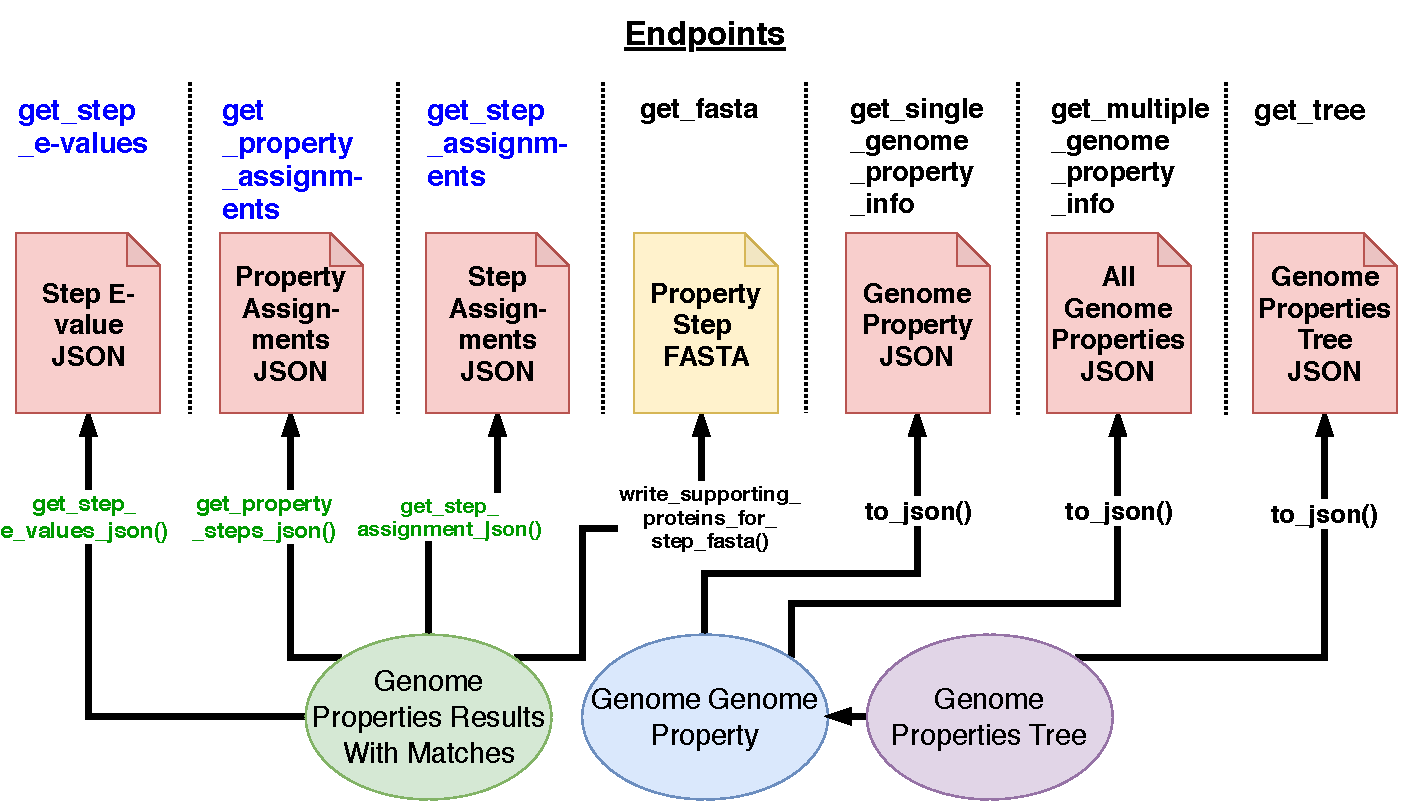
\includegraphics[width=\textwidth]{media/micromeda-server-new-endpoints.pdf}
	 \caption{New endpoints returning of step assignments, step supporting information and property assignments could be created (blue). These new endpoints could be supported by new JSON generating methods of GenomePropertiesResultsWithMatches objects (green).}
	 \label{fig:new_endpoints}
\end{figure}

\subsection{Creation of an Endpoint for Returning Domain Annotation Supporting Property Steps} \label{e-value-endpoint}

Micromeda files not only contain property and step assignments for a set of organisms but also contain additional information such as domain annotations and proteins sequences that support the existence of property steps. Micromeda-Server currently provides an endpoint for accessing protein sequences that support steps (see Subsection \ref{get-fasta-endpoint}). However, there are no endpoints for accessing the stored InterProScan annotations of these proteins. Specifically, these annotations contain E-value scores representing how closely the domain in the protein matches to a model of a representative domain in a protein database (see Section XXX). The E-value scores for these domains may be useful for client visualizations that compare not only the presence and absence of proteins which support property steps but also compare how close these matches are to existing domain models. Thus, it may be useful to create a new endpoint which returns domain annotation E-value scores for domains which support property steps (Fig. \ref{fig:new_endpoints}). This endpoint could generated its data from the \textbf{step\_matches} DataFrame of reconstituted GenomePropertiesResultsWithMatches objects.

\subsection{Containerization of Micromeda-Server for Increased Deployability}

The deployment strategy discussed in Section \ref{micromeda-server-deployments} requires the deployment of multiple pieces of software alongside Micromeda-Server, such as Redis caching servers or larger web servers such as NGINX. The set-up and configure of such software is complex, time-consuming, and error-prone. One potential solution for automating such complex deployments is software containerization \cite{syed2015software} (see \href{en.wikipedia.org/wiki/OS-level\_virtualisation}{en.wikipedia.org/wiki/OS-level\_virtualisation}) and infrastructure as code (IaC) \cite{artac2017devops} (see \href{en.wikipedia.org/wiki/Infrastructure\_as\_code}{en.wikipedia.org/wiki/Infrastructure\_as\_code}). 

Software, such as Micromeda-Server, often require an interpreter \cite{bennett1952interpretative} (see \href{en.wikipedia.org/wiki/Interpreter\_(computing)}{en.wikipedia.org/wiki/Interpreter\_(computing)}) to run their Python code and also require various third-party software libraries. In the case of Micromeda-Server, these libraries would be Flask and Pygenprop. These dependencies are often required to be at specific versions. If different software elements on a server computer system share the same dependencies, such as interpreters or libraries, there may be conflicts. If one software requires a shared dependency at a specific version and, if updated, this dependency may break the other software on the system. As a specific example, Python software often requires a Python interpreter at version 2.7, whereas others require an interpreter at version 3.4 or higher. Updating a globally installed Python interpreter to version 3.4 will break software that requires version 2.7. 

One potential solution to this dependency problem is software containerization. In this technique, a slice, called a container, of host operating system's memory and process space is partitioned into its own space. From the perspective of the software running in this new slice, it looks like it is running in a freshly installed version of the host operating system. A new copy of the software, such as Micromeda-Server, and new copies of its dependencies can then be installed within this slice. These copies are entirely independent of and sheltered from the other software running on the host computer system and can run without conflict. Even more complex containerization systems, such as Docker (\href{docker.com}{docker.com}), provide these slices with their disk and network spaces. Rather than multiple software and dependencies that need to be installed in series, containers and the software inside can be installed using a single pre-built binary that can be downloaded by users from repositories such as Docker Hub (\href{hub.docker.com}{hub.docker.com}). Afterwards, such containers can be started in only a few commands. It is common to place different software servers in separate containers. For example, Micromeda-Server could be placed in one container and the Redis server it relies upon could be placed in another (Fig. \ref{fig:micromeda-docker}). 

IaC systems, such as Docker Compose (see \href{docs.docker.com/compose}{docs.docker.com/compose}), can be used to write scripts that combine multiple types of containers, containing different software components, into larger systems. For example, a Docker Compose script could be written for each type of deployment in Section \ref{micromeda-server-deployments} and these scripts could be run on new server computer systems or developer machines to quickly install Micromeda-Server and dependencies (Fig. \ref{fig:micromeda-docker}). Container orchestration systems \cite{tosatto2015container}, such as Kubernetes (\href{kubernetes.io}{kubernetes.io}), can be installed on clusters of server computer systems and allow for the installation of complex deployments, such as the multi-server deployment described in Subsection \ref{multi-server-micromeda-deployment}. Kubernetes can take an IaC Docker Compose script and ensure that different containers, containing different pieces of software, are spread across the cluster and correctly networked together. Creation of Docker containers and Docker Compose scripts for Micromeda-Server could vastly increase its ease of install.

\begin{figure}[!ht]
  \centering
	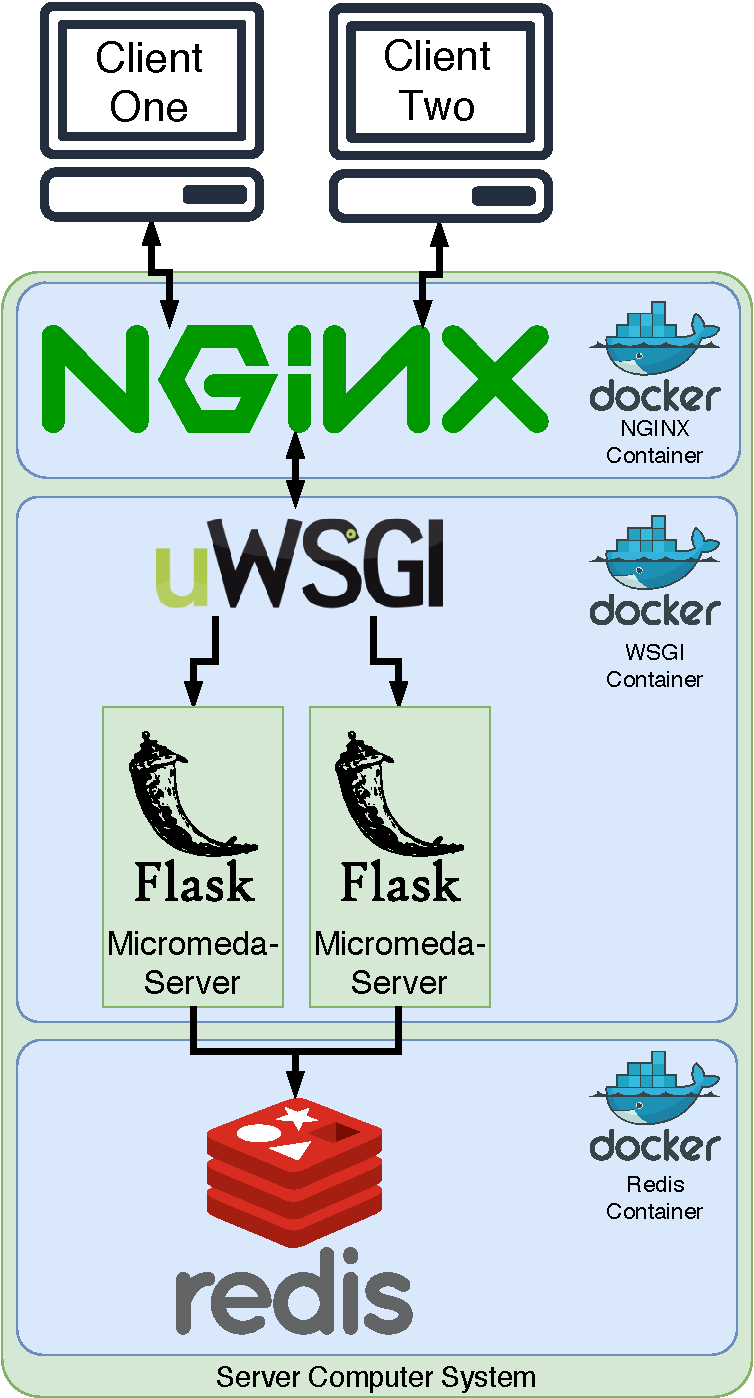
\includegraphics[width=0.55\textwidth]{media/micromeda-server-docker.pdf}
	 \caption{Docker could be used to containerize different components of Micromeda-Server. Docker Compose scripts could be used to ensure that each of these containers is generated in the right order. For example, by starting the Redis server before the uWSGI server.}
	 \label{fig:micromeda-docker}
\end{figure}

\section{Summary}

The creation of web server API's for accessing information about biochemical pathways, and even the precalculated presence and absence of these pathways across organisms, is quite common \cite{wu2006kobas,moriya2010pathpred,pireddu2006path,vallenet2009microscope,aziz2008rast,takami2016automated,moriya2007kaas,chou2009fmm}. Indeed, such web APIs have been developed by both the creators of KEGG \cite{kawashima2003kegg} and Metacyc \cite{karp2013data}, not only for their web client applications but also for academic use. A web server has also been built for EBI's Genome Properties database website \cite{richardson2018genome}. However, its API is not publicly available and is only designed to support the Genome Properties website. The KEGG, Metacyc, and Genome Properties website all contain precalculated pathway annotations for sets of reference organisms \cite{kanehisa2000kegg,karp2002metacyc,karp2013data}. With the exception the Genome Properties website, these websites \cite{kanehisa2016blastkoala}, or similar sites that use their databases \cite{chou2009fmm,moriya2007kaas,takami2016automated}, can pathway annotate user-supplied genomes uploaded in FASTA format \cite{pearson19905}. Such annotation servers are complex to build and host due to the relative computational complexity of scanning for genes that support the existence of pathway steps. In contrast, the Genome Properties website allows for the upload of user-created InterProScan annotation files. The creation of such annotations files pushes the most computationally complex part of the Genome Properties pipeline, domain annotation, off onto end-users \cite{richardson2018genome}. As discussed in Chapter XXX, Micromeda-Server follows a similar approach. However, unlike the Genome Properties website, Micromeda-Server takes the upload of Micromeda files. The use of Micromeda files provides a unique advantage to Micromeda-Server, in contrast to almost all other annotation servers, because it allows users to download information about supporting proteins and domain annotations if such an endpoint was created and used in pathway determination. Micromeda files also allow the upload of datasets consisting of pathway annotations from hundred of genomes simultaneously, unlike other pathway servers, which often require uploading genomes or InterProScan annotations for organisms one at a time. With the avoidance of computationally complex annotation steps and a variety of horizontally scalable deployment options, Micromeda-Server should provide a reliable and sustainable API for Micromeda's client application.
